\documentclass[10pt,twocolumn,a4paper]{article}
\usepackage[margin=0.68in,top=0.65in,bottom=0.7in]{geometry}
\usepackage[utf8]{inputenc}
\usepackage[T1]{fontenc}
\usepackage{mathptmx}
\usepackage{amsmath,amssymb,bm}
\usepackage{graphicx,booktabs,tabularx,array,multirow}
\usepackage{microtype,cite}
\usepackage{caption}
\captionsetup{font=small,labelfont=bf,labelsep=period}
\usepackage{xcolor}
\definecolor{ink}{HTML}{172C43}
\definecolor{accent}{HTML}{007C83}
\usepackage{hyperref}
\hypersetup{colorlinks=true,urlcolor=accent,citecolor=ink,linkcolor=ink,pdftitle={Temporal Retiming Attacks on Hybrid Quantum Spiking Classifiers}}
\usepackage{url}
\urlstyle{same}
\Urlmuskip=0mu plus 2mu\relax
\makeatletter
\g@addto@macro\UrlBreaks{\do\-\do\_\do\?\do\&\do\=}
\makeatother
% Keep one bibliography entry together across columns/pages.
\let\originalthebibliography\thebibliography
\renewcommand{\thebibliography}[1]{\originalthebibliography{#1}\interlinepenalty=10000\relax}
\newcolumntype{L}{>{\raggedright\arraybackslash}X}
\newcolumntype{C}{>{\centering\arraybackslash}X}
\newcolumntype{R}{>{\raggedleft\arraybackslash}X}
\setlength{\emergencystretch}{1.5em}
\raggedbottom
\setlength{\columnsep}{0.25in}
\setlength{\textfloatsep}{11pt plus 2pt minus 2pt}
\setlength{\dbltextfloatsep}{12pt plus 2pt minus 2pt}
\setlength{\floatsep}{9pt plus 2pt minus 2pt}
\renewcommand{\topfraction}{0.95}
\renewcommand{\dbltopfraction}{0.95}
\renewcommand{\textfraction}{0.05}
\renewcommand{\floatpagefraction}{0.85}
\setcounter{topnumber}{3}
\setcounter{dbltopnumber}{2}

\pagestyle{plain}
\begin{document}
\twocolumn[{
\begin{center}
{\LARGE\bfseries Temporal Retiming Attacks on\\[3pt]
Hybrid Quantum Spiking Classifiers\par}
\vspace{9pt}
{\normalsize Author names withheld for review\par}
\vspace{12pt}
\end{center}
\begin{minipage}{\textwidth}
\small\textbf{Abstract.} Event timing is an adversarial input dimension, but attack comparisons depend on both the feasible retiming and the computation allocated to the search. We study this issue in QSNN-v3, an implemented hybrid of a classical Conv/LIF frontend and an analytically simulated eight-qubit probability readout. The model achieves 97.272\% $\pm$ 0.212\% validation accuracy across five seeds conditional on shared pretraining and split. On 100 jointly clean-correct seed-42 validation examples, timestamp PGD succeeds on three examples at each tested radius. Derivative-free margin search produces zero to two additional successes depending on candidate, forward-pass or elapsed-time matching; no paired comparison establishes significant superiority. Separate classical packet-grid controls show that similar clean accuracy can accompany sharply different outcomes under one attack recipe, without isolating a representation or quantum effect. The evidence supports protocol-specific temporal vulnerability; official-test hybrid robustness and a quantum-specific mechanism remain unmeasured.
\par\vspace{5pt}\textbf{Keywords:} event-driven classification; adversarial retiming; hybrid quantum classifiers; spiking neural networks; matched attack evaluation.
\end{minipage}
\vspace{16pt}
}]
\section{Introduction}\label{sec:introduction}
Event-driven classifiers process not only where an event occurs but when it occurs. Retiming can change a prediction while preserving event identities, spatial coordinates, polarity and total count. Surrogate-gradient learning makes spiking dynamics trainable \cite{neftci2019}, while spike-retiming attacks make timing an explicit adversarial input dimension \cite{yu2026}. An evaluation must therefore specify both the admissible temporal changes and the computation available to find them.

We investigate end-to-end temporal vulnerability in an implemented hybrid classifier, emphasizing how computational matching changes attack comparisons and why results from separate temporal representations require separate interpretation. Our primary target, QSNN-v3, maps events through a classical Conv/LIF frontend, learned angles, an eight-qubit circuit and an affine probability readout. The central question is whether conclusions about its observed attack outcomes change with the definition of matched computation. Candidate count, forward-pass count and elapsed time measure different resources, particularly when only one attack uses gradients.

On the same 100 joint clean-correct validation examples, timestamp PGD causes three hybrid failures at each tested radius. TEMP-DRIFT-v2, a derivative-free margin search, causes 3--5 depending on radius and computational control. The largest numerical difference occurs under elapsed-time matching; no paired test establishes superiority. A separate four-model classical packet-grid study supplies context: similar clean accuracy need not imply similar attack outcomes. Differences in victims, populations, checkpoints and budget units prevent a causal representation ablation or a pooled robustness ranking across these studies.

The evaluation concerns the implemented composition. Quantum-classifier robustness can depend on encoding, model structure and adversarial access \cite{wendlinger2024comparative,gong2024randomized,dowling2026guarantees}; here the perturbation enters before the classical frontend. The following concrete outputs organize the paper:
\begin{enumerate}
\item \textbf{An explicit hybrid attack interface.} We specify temporal aggregation, Conv/LIF features and the sole quantum-probability readout, with preserved implementation evidence and a readout-specific margin observation. Missing artifacts limit full reproduction.
\item \textbf{Paired computational comparisons.} We report success counts, overlaps, exact paired tests and resource accounting for candidate, forward and elapsed-time controls on a frozen timestamp population.
\item \textbf{Classical interpretation controls.} We compare four architectures under a common packet-retiming recipe to delimit what clean accuracy and one optimizer establish.
\end{enumerate}
Source labels [R1]--[R10] map to preserved repository reports and code in the supplement. The supplement also retains development studies, full numerical tables and the conceptual literature comparison.

\section{Related work}\label{sec:related}
\paragraph{Raw-event attacks and constrained retiming.}
Surrogate-gradient learning provides a practical route through the nondifferentiable dynamics of spiking networks \cite{neftci2019}. B\"uchel et al. study event additions and removals in spiking vision models \cite{buchel2022attacks}, a different feasible set from identity-preserving retiming. An attack on an aggregated tensor and an attack on the underlying event stream need not have the same feasible set. Yao et al. attack raw event data using a probabilistic treatment of discrete event values and sparsity control \cite{yao2024rawevent}. Their construction permits event-value and support changes, whereas our native-event threat model preserves event identities, coordinates, polarities and count. Du et al. investigate raw-event attacks with configurable latencies \cite{du2026latencies}, providing a particularly relevant connection to temporal manipulation. These works motivate attacks at the event interface without making their constraints interchangeable with ours.

\paragraph{Capacity constraints and representation-specific budgets.}
Yu et al. formalize capacity-one spike retiming and budgets on maximum displacement, total delay and the number of retimed spikes \cite{yu2026}. Our classical packet-grid comparison uses a local implementation of this framework, with completed results for maximum displacement and retimed-packet count. The native-timestamp experiment instead permits multiple events to contribute to a frame cell. Its duration-scaled timestamp radius cannot be identified with a one-bin packet displacement. We consequently compare attacks within each stated regime and do not rank the regimes by their raw ASR values.

\paragraph{Hybrid spiking and quantum models.}
Quantum temporal models encompass distinct computational constructions. Brand and Petruccione develop a quantum leaky integrate-and-fire neuron and network \cite{brand2024}; Jha et al. combine SNN-derived EEG features with quantum-kernel classification \cite{jha2025hybrid}; and SPATE studies spike-derived temporal quantum encodings \cite{spate2026}. QSNN-v3 instead composes classical Conv/LIF dynamics, a learned angle map, a data-re-uploading variational circuit \cite{perez2020}, and a linear classifier on the complete measurement-probability vector. These differences concern the model and interface, so accuracy or security claims do not transfer directly between the constructions.

\paragraph{Adversarial robustness of quantum classifiers.}
Wendlinger et al. compare quantum and classical classifiers using transfer attacks, perturbation structure and Lipschitz-based analysis \cite{wendlinger2024comparative}. Gong et al. investigate randomized encodings under specified adversarial-access assumptions \cite{gong2024randomized}, while Dowling et al. establish robustness guarantees for particular quantum-classifier settings \cite{dowling2026guarantees}. Khatun and Usman use classical autoencoders to distill quantum adversarial manipulations on image benchmarks \cite{khatun2025distillation}; this is neither an implemented defense here nor evidence for temporal-retiming protection. These studies motivate stating the encoding and adversary explicitly. Their guarantees and defenses cannot be assigned to QSNN-v3 without checking the corresponding assumptions, especially because our perturbation enters before a classical event-processing frontend.

\paragraph{Evaluation strength and computational controls.}
PGD is a standard iterative baseline \cite{madry2018}, but the failure of one optimizer is insufficient evidence of robustness \cite{carlini2019,athalye2018obfuscated}. Diverse attacks and improved optimization can expose failures missed by an individual configuration \cite{croce2020reliable}. We therefore report paired outcomes under candidate, forward-pass and elapsed-time controls. These controls answer different resource questions and do not establish optimality of either attack. Standard image-space attack ensembles also require adaptation before they respect our order, timing and packet constraints.


The supplementary conceptual-positioning table distinguishes these interfaces without ranking external ASRs.

\section{Models and representations}\label{sec:model}
Figure~\ref{fig:overview} summarizes the two retiming regimes and the implemented hybrid pipeline.
\subsection{Native events and temporal-grid packets}
The timestamp study uses native N-MNIST events $e_i=(x_i,y_i,p_i,t_i)$. Event identities, coordinates, polarity, labels and event count are immutable. Timestamps are assigned to ten equal-duration bins using the clean recording endpoints. The differentiable adapter has hard count accumulation in the forward pass and triangular interpolation weights for the backward pass. Counts are capped at 255 by the adapter. The hybrid frontend then applies $\min(X/8,1)$. These input transformations are model preprocessing; the preservation claim refers to the underlying events.

The grid study instead freezes a ten-bin equal-event-count representation. Each nonzero cell on a fixed spatial/polarity line is one amplitude-bearing packet. A binary packet has value one; an integer packet carries its complete cell count. A packet with count five remains a single packet carrying five during retiming. Collision-free capacity-one projection prevents packet splitting, merging, deletion, creation and amplitude changes. This distinction matters because multiple raw events can occupy one cell in the timestamp study, while one grid packet is indivisible in the second study.


\subsection{The implemented hybrid classifier}
The Conv/LIF extractor uses two $3\!\times\!3$ bias-free convolutions with 16 and 32 output channels, batch normalization and average pooling. LIF dynamics use decay 0.5. Time-averaged spike activations and the final membrane state are pooled to $4\!\times\!4$ spatial summaries and concatenated. A learned projection followed by tanh produces 32 latent features. A learned 32-to-8 projection and another tanh feed the circuit head. An additional learned 8-to-8 projection, initialized to the identity, produces bounded rotation angles.


For the latent vector $h\in\mathbb{R}^{32}$, the learned angle map is
\begin{equation}\label{eq:angles}
\begin{aligned}
 u&=\tanh(W_{32}h+b_{32}),\\
 a&=\pi\,\operatorname{clip}(W_8u+b_8,-1,1).
\end{aligned}
\end{equation}
The eight-qubit register starts in $|0\rangle^{\otimes 8}$. Each of two blocks applies an RY upload of each angle, an RZ upload scaled by a learned phase parameter, learned RY/RZ gates, and a ring of CNOT gates. Learned local RZ/RY rotations set the measurement basis. The model returns all 256 computational-basis probabilities to a linear ten-class classifier. All paths from the latent features to the logits pass through the circuit; there is no direct latent-to-logit branch.


\begin{equation}\label{eq:readout}
\begin{aligned}
p_k&=\left|\langle k|U_{\theta}(a)|0\rangle^{\otimes 8}\right|^2,
&& k=0,\ldots,255,\\
z&=W_{\mathrm{out}}p+b_{\mathrm{out}}.
\end{aligned}
\end{equation}
The backend is an analytic batched PyTorch state-vector simulation with complex64 amplitudes. Probabilities are computed exactly within numerical precision. The experiments do not involve quantum hardware, finite-shot readout or hardware noise. The name QSNN-v3 identifies this hybrid implementation and should not be interpreted as a network of physical quantum LIF neurons [R1].

\begin{table}[t]
\centering\caption{Trainable parameters of QSNN-v3.}\label{tab:parameters}
\small\begin{tabularx}{\linewidth}{L R}\toprule
\textbf{Component} & \textbf{Parameters}\\\midrule
Conv/LIF frontend and 32D summary & 37,792\\
Learned $32\to 8$ projection & 264\\
Angle map and quantum head & 136\\
Probability-to-logit classifier & 2,570\\\midrule
\textbf{Total} & \textbf{40,762}\\\bottomrule
\end{tabularx}
\vspace{3pt}\begin{minipage}{\linewidth}\footnotesize
The quantum head includes the learned $8\to8$ angle map, two upload blocks and learned measurement basis. Nontrainable BatchNorm buffers and state-vector storage are excluded [R1].
\end{minipage}\end{table}
\begin{figure*}[t]
\centering
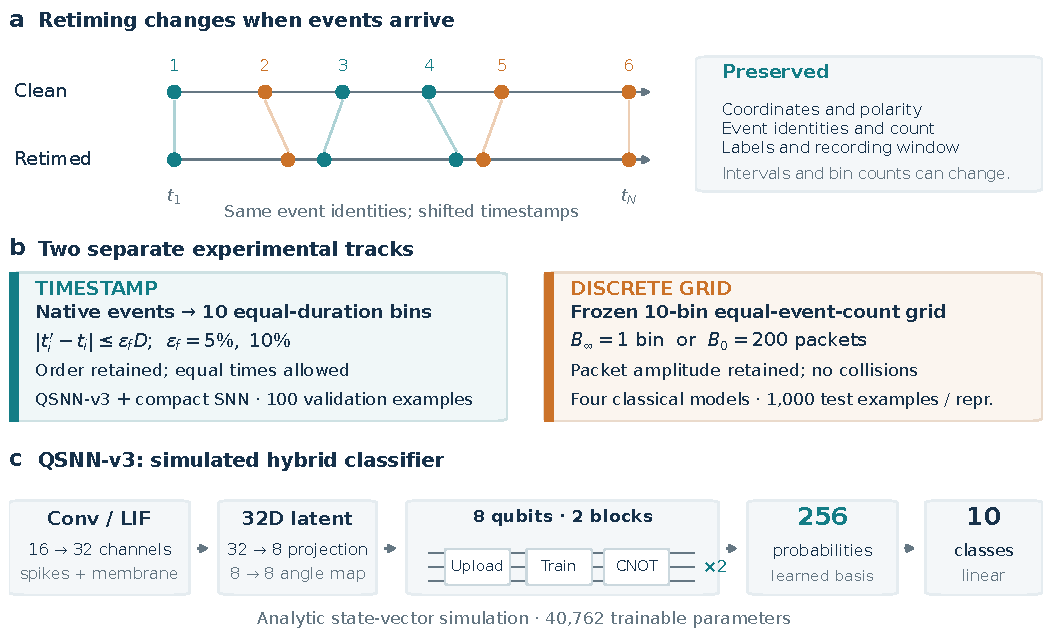
\includegraphics[width=\textwidth]{figures/fig01_overview.pdf}
\caption{Retiming protocols and implemented QSNN-v3. (a) Schematic retiming preserves event identity, coordinates, polarity, labels and count; intervals and bin counts can change. (b) The timestamp and discrete-grid studies use different representations, populations and budget units. Timestamp perturbations preserve nondecreasing order within the clean recording window; grid perturbations preserve indivisible packet amplitudes with collision-free scheduling. (c) Conv/LIF summaries pass through 32 latent features, learned 32-to-8 and 8-to-8 maps, and an eight-qubit, two-block circuit. The 256-probability readout alone feeds the ten-class classifier. The 40,762-parameter model uses analytic state-vector simulation. Circuit and event drawings are schematic. Sources: [R1--R4].}\label{fig:overview}
\end{figure*}

\subsection{State distance and classification margin}
\label{sec:margin_interpretation}
For the fixed trained model, let $\rho$ and $\rho'$ denote the clean and retimed quantum states before the fixed readout measurement, and let $q,q'\in\mathbb{R}^{256}$ be the corresponding outcome-probability vectors. Write the logits as $z(q)=Wq+b$, and define the clean pairwise margin against class $k\ne y$ by
\begin{equation}
m_{yk}(q)=(w_y-w_k)^\top q+b_y-b_k.
\end{equation}
Here $y$ is the clean predicted class, equal to the label on the attacked clean-correct subset, and $w_k$ is row $k$ of $W$. Measurement cannot increase trace distance, hence
\begin{equation}
\tfrac12\|q-q'\|_1\leq D_{\mathrm{tr}}(\rho,\rho'),
\qquad
D_{\mathrm{tr}}(\rho,\rho')=\tfrac12\|\rho-\rho'\|_1.
\end{equation}
The state norm is the trace norm; for probability vectors it is the ordinary $\ell_1$ norm. Combining this inequality with H\"older's inequality gives
\begin{equation}
\begin{split}
m_{yk}(q')\geq m_{yk}(q)\\
{}-2\|w_y-w_k\|_\infty D_{\mathrm{tr}}(\rho,\rho').
\end{split}
\label{eq:state_margin}
\end{equation}
Thus a sufficient condition for retaining class $y$ is that the right-hand side remain strictly positive for every $k\ne y$. To see this, subtract the two affine margins and bound the resulting inner product by $\|w_y-w_k\|_\infty\|q'-q\|_1$; positivity of all pairwise margins then preserves the argmax.

This observation separates state displacement from decision failure. A larger state distance need not cause a label change, and a small clean margin can make a smaller displacement consequential. Equation~\eqref{eq:state_margin} is a conditional interpretation of the implemented readout, not a certified timestamp radius: no uniform bound from admissible event retiming through the classical frontend to $D_{\mathrm{tr}}$ has been established here. The final-model campaign also does not report the per-example states needed to evaluate this condition. Its connection to quantum robustness theory is therefore conceptual rather than an application of an existing certificate \cite{dowling2026guarantees}.

\section{Threat models and attacks}\label{sec:attacks}
\subsection{Timestamp retiming}
We consider untargeted test-time evasion. For a sorted clean timestamp vector t, the feasible retiming keeps each event within its clean timestamp neighborhood and within the recording endpoints, and preserves a nondecreasing sequence. If D is the clean duration, the perturbation budget is $\epsilon$ = $\epsilon_f$ D. The reported matched comparisons use $\epsilon_f$ = 0.05 and 0.10. Equal timestamps are permitted; capacity-one grid occupancy is not part of this threat model.


\begin{equation}\label{eq:feasible}
\begin{gathered}
|t_i'-t_i|\leq\epsilon_f D,\qquad t_1\leq t_i'\leq t_N,\\
 t_i'\leq t_{i+1}',\qquad D=t_N-t_1+1.
\end{gathered}
\end{equation}
The extra unit in $D$ follows the implementation's inclusive timestamp convention.
The implementation first clips a candidate to eventwise intervals, applies a cumulative maximum, and clips to the recording range. We describe this as a feasibility operator, not as the Euclidean projection onto the constrained set. Event counts over the fixed recording window are preserved. Inter-spike intervals, time-bin counts and detector statistics can change. No completed final-model experiment establishes statistical indistinguishability from clean inputs.


\paragraph{Timestamp PGD.}
Timestamp PGD uses white-box gradients of cross-entropy through the hard-forward/soft-backward frame adapter and the surrogate-gradient LIF model. It starts at the clean timestamps, takes 20 sign-gradient steps with step size $\epsilon$/5, and applies the feasibility operator after every step. The candidate with the highest cross-entropy among the clean input and 20 iterates is retained. There is no random start in the preserved implementation [R2]. Selection does not explicitly retain any successful intermediate candidate: a higher-cross-entropy candidate may still be correctly classified. This is a verified selection rule, not evidence that a reported success was lost; testing its empirical effect requires the missing trajectories.


\begin{equation}\label{eq:pgd}
\begin{aligned}
g^{(k)}&=\operatorname{sign}\!\left(\nabla_t\mathrm{CE}(z(t^{(k)}),c)\right),\\
t^{(k+1)}&=\Pi_{\epsilon}\!\left[t^{(k)}+\frac{\epsilon}{5}g^{(k)}\right].
\end{aligned}
\end{equation}
\paragraph{TEMP-DRIFT-v2.}
TEMP-DRIFT-v2 is a derivative-free search using model logits and the true label. It minimizes the true-class margin. A negative margin indicates that a competing logit exceeds the correct-class logit. This objective is a classification objective and contains no fidelity, density-matrix distance or classical-statistics penalty.


\begin{equation}\label{eq:margin}
\min_{t'\in\mathcal{F}_{\epsilon}} m(t'),\qquad
m(t)=z_c(t)-\max_{j\neq c}z_j(t).
\end{equation}
The preserved full-budget implementation evaluates 600 uniformly perturbed feasible candidates. It retains the 12 candidates with lowest margin, then runs four generations of 250 children. Each child combines an elite parent, half the difference between two elite candidates and Gaussian noise at scales 0.50, 0.30, 0.18 and 0.10 times $\epsilon$. Every proposal is made feasible before evaluation. The final candidate with lowest margin is returned. This configuration uses 1,600 candidate evaluations [R2]. The matched implementation uses 13 initial candidates plus four generations of two children for $Q=21$, and 13 plus four generations of seven for $Q=41$. It always keeps 12 elites; the four noise scales are unchanged. For elapsed-time budgets it sets $n_0=\max(12,\operatorname{round}(0.375Q))$ and $n_g=\operatorname{round}((Q-n_0)/4)$, recording the actual total $n_0+4n_g$. The selected $Q=4{,}000$ and $1{,}600$ give $1{,}500+4\times625$ and $600+4\times250$, respectively. The supplement gives the complete schedule and pseudocode [R3].


A finite search need not find more successes at a larger allowed radius; the observed 4-to-3 decrease under access matching is not evidence of a smaller feasible set. Each reported radius is a standalone search. Any future cumulative best-so-far curve must count the earlier searches and warm starts. TEMP-DRIFT-v2 is the historical implementation name; throughout the final timestamp comparison it denotes margin search.

\paragraph{Inference state.}
Both timestamp victims are loaded in evaluation mode, fixing BatchNorm statistics. Their forward methods initialize membrane and output accumulators locally on every call; the preserved code has no cross-candidate persistent neuron state. The recovered grid reference forwards also call \texttt{reset\_net}; this is static evidence, not a batching/order/reset experiment on the saved victims.

\subsection{Discrete packet retiming}
In the second study, let $s_i$ and $s_i'$ denote a source packet bin and its destination. Budgets count packet displacements independently of amplitude. A packet carrying amplitude five and shifted by two bins contributes two to $B_1$ and one to $B_0$. Capacity-one projection preserves packet identity, amplitude, event line and total represented mass.


\begin{equation}\label{eq:budgets}
\begin{aligned}
B_{\infty}&=\max_i|s_i'-s_i|, & B_1&=\sum_i|s_i'-s_i|,\\
B_0&=\sum_i\mathbf{1}[s_i'\neq s_i].
\end{aligned}
\end{equation}
The local projected-in-the-loop attack uses differentiable shift probabilities and evaluates feasible hard schedules. Only $B_\infty$ = 1 and $B_0$ = 200 are complete in the controlled four-model campaign [R4]. The recovered adapter selects the pinned upstream L0 class, whose loss hard-codes a normalized budget-penalty coefficient of five. Its separate capacity penalty is \texttt{lambda\_cap=20}; the constructor default \texttt{lambda\_B=0} does not set the hard-coded coefficient. The report compares five with the reference description of ten [R4]. This source-level finding does not reconstruct the historical runtime configuration. Historical sweeps from other checkpoints appear in the supplement.

\section{Experimental protocol}\label{sec:protocol}
\subsection{Training and model selection}
N-MNIST contains event recordings of handwritten digits \cite{orchard2015}. The hybrid campaign uses a frozen stratified partition of 55,000 training and 5,000 validation examples from the official training set. Architecture selection was performed with seed 42 and validation data. The chosen wide4 frontend and project\_measure2 circuit were then held fixed across model seeds 42, 123, 777, 2026 and 6543. The official test partition was not instantiated for the final QSNN campaign [R1]. Consequently, its reported clean accuracy is validation accuracy after model selection.

All five hybrid runs load the same hash-verified, seed-42 classical frontend checkpoint. The frontend is frozen for the first two epochs, then optimized with its BatchNorm layers kept in evaluation mode. The random seeds vary subsequent initialization and training stochasticity; they do not represent five independently pretrained frontends or five data splits. This conditional design limits the scope of the reported between-seed standard deviation.


Training uses AdamW with weight decay $10^{-4}$ and batch size 256 for at most 40 epochs. Learning rates are $5\times10^{-5}$ for the extractor, $2.5\times10^{-4}$ for the projection/circuit, and $10^{-3}$ for the classifier. A ReduceLROnPlateau scheduler uses factor 0.5, patience 2 and minimum rate $10^{-5}$. The highest validation accuracy selects a checkpoint, with validation loss breaking ties; early stopping uses patience 6 after at least eight epochs. Gradients are clipped at norm 1. The frontend uses float16 autocast; circuit inputs and amplitudes use float32 and complex64. Seed 42 was externally interrupted during epoch 38; its saved epoch-37 checkpoint was re-evaluated [R1].

\subsection{Populations and attack budgets}
The timestamp protocol freezes 100 validation examples, with ten examples per class, correctly classified by both models before attack. It reuses their identities across conditions. This joint-correct restriction permits paired attack comparisons but excludes examples that only one model classifies correctly. It is not a population-wide robust-accuracy estimate. The compact SNN checkpoint in this study differs from the retrained custom-SNN checkpoint in the controlled grid study.

PGD evaluates 21 candidate timestamps, including the clean candidate. Its implementation makes 41 attack-internal forward passes and 20 backward evaluations because candidate scoring and gradient computation use separate forwards. TEMP uses Q forward evaluations and no backwards. The first matched condition gives TEMP 21 candidates; the second gives it 41 forwards. Neither converts a backward pass into an assumed number of forward passes. Verification adds two forwards per new record and is excluded from attack timing.

Elapsed-time calibration selects Q = 4,000 for QSNN and Q = 1,600 for SNN. The reported median TEMP/PGD timing ratios are 0.978 and 1.083, respectively [R3]. Candidate matching, forward matching and elapsed-time matching answer different computational questions. Exact equality of elapsed time is not asserted, and no throughput or latency claim is inferred from the ratios alone.

The controlled grid campaign trains four architectures under a common local recipe, data split, seed, optimizer settings and validation-selected checkpoint rule [R4]. For each representation it selects the first 1,000 official-test examples that all four models classify correctly. The joint-correct pools contain 9,522 binary and 9,495 integer examples. Within each representation the same frozen manifest is used for every architecture and budget. The two representations use different manifests.


\begin{table*}[t]\centering
\caption{Experimental populations and budget units. These regimes are analyzed separately.}\label{tab:populations}
\small\begin{tabularx}{\textwidth}{>{\raggedright\arraybackslash}p{.15\textwidth}L L >{\raggedright\arraybackslash}p{.21\textwidth}}\toprule
\textbf{Study} & \textbf{Models} & \textbf{Attack population} & \textbf{Budget}\\\midrule
Native timestamps & QSNN-v3 and compact SNN & 100 common clean-correct validation examples; 10/class; seed 42 & $\epsilon_f\in\{0.05,0.10\}$ of recording duration\\
Controlled grid & Custom SNN, ConvNet, spiking ResNet18, VGGSNN & First 1,000 common clean-correct official-test examples per representation; seed 42 & $B_\infty=1$ bin or $B_0=200$ packets\\
Supporting studies & Earlier models/checkpoints & Study-specific subsets stated in the supplement & Study-specific timing or packet budgets\\\bottomrule
\end{tabularx}
\vspace{3pt}\begin{minipage}{\textwidth}\footnotesize
The compact timestamp SNN and retrained grid custom SNN are different checkpoints. Binary and integer grid attacks use separate manifests, drawn from joint-correct pools of 9,522 and 9,495 test examples, respectively [R2--R5].
\end{minipage}\end{table*}

\subsection{Metrics, paired tests and evidence}
Clean accuracy is measured on the stated complete validation or test partition. Attack success rate (ASR) is conditioned on clean correctness. In joint-model studies the denominator is the shared clean-correct subset. A success is an untargeted misclassification after retiming.


ASR is conditional on the stated clean-correct attack population. Consequently, $1-\mathrm{ASR}$ describes survival under the evaluated attack on that selected population; it is not an unconditional robust accuracy on the full validation or test set. Reusing a joint-correct population improves within-study comparability but changes the estimand relative to evaluation on all examples.

For the stated clean-correct attack population $\mathcal{P}$, we use
\begin{equation}\label{eq:asr}
\operatorname{ASR}(\mathcal{P})=
\frac{1}{|\mathcal{P}|}\sum_{i\in\mathcal{P}}\mathbf{1}\!\left[f(X_i')\neq y_i\right].
\end{equation}
We report arithmetic means and sample standard deviations across the stated model seeds. For paired timestamp comparisons, $b$ counts examples broken only by PGD and $c$ counts examples broken only by TEMP. The exact two-sided McNemar test uses a $\operatorname{Binomial}(b+c,1/2)$ null distribution, with $p=1$ for $b+c=0$. It assesses observed paired discordance, not equality of all possible attack strengths. Reused examples across seeds and conditions are not treated as independent additional subjects.

All numerical results are taken from preserved reports and source files at repository snapshot \texttt{80d02f5733d4} \cite{repository}; the full commit identifier is recorded in the supplement. We checked parameter arithmetic, aggregate statistics, paired counts and exact paired $p$-values. Model execution and per-example bootstrap resampling were not repeated. Missing raw outputs and provenance boundaries are documented in Sec.~\ref{sec:discussion} and the supplement.

\section{Results}\label{sec:results}
The completed evidence consists of three distinct components: a frozen five-seed QSNN-v3 validation campaign, a seed-42 paired native-timestamp attack comparison, and a seed-42 four-model packet-grid study. We report their denominators and computational definitions separately. Percentages below are conditional on the stated split and, for ASR, the stated clean-correct population; no result is reconstructed for an uncompleted experiment.

\subsection{Clean validation of the hybrid classifier}
The frozen QSNN-v3 configuration achieves 97.2720\% $\pm$ 0.2119\% validation accuracy and a reported macro-F1 of 97.2736\% $\pm$ 0.2119\% across five training seeds. Individual accuracies are 97.06\%, 97.28\%, 97.52\%, 97.44\% and 97.06\% for seeds 42, 123, 777, 2026 and 6543, respectively; the descriptive span is 0.46 percentage points. The preserved SNN validation reference has 98.1320\% $\pm$ 0.2407\% accuracy, giving a descriptive QSNN-minus-SNN difference of -0.8600 percentage points. A matched validation-F1 comparison is unavailable.

The five hybrid runs share one pretrained seed-42 frontend and one 55,000/5,000 training/validation split. The architecture and training configuration were frozen after seed-42 development. Thus, the sample standard deviation measures subsequent training variation conditional on shared pretraining and data, rather than five independently pretrained pipelines. The selected epochs are 37, 24, 40, 38 and 40. The seed-42 process was externally terminated during epoch 38; its saved epoch-37 checkpoint was reloaded and evaluated for the reported result.

The seed-42 wide4 classical frontend reaches 97.80\% validation accuracy with 38,122 parameters, while its selected hybrid continuation reaches 97.06\% with 40,762 parameters. The 0.74-point accuracy difference and 2,640 added parameters are descriptive: differing training stages and budgets prevent attribution to an isolated circuit component. All final QSNN clean results are validation results; the official test partition was not accessed. The campaign establishes an accurate implemented hybrid victim, rather than a quantum accuracy advantage.

Figure~\ref{fig:matched}a shows the individual runs and their conditional mean and sample standard deviation. Table~\ref{tab:validation} gives the selected checkpoint epochs; full per-run training records are retained in the supplement.
\begin{table}[t]\centering
\caption{QSNN-v3 validation on the same 5,000 examples.}\label{tab:validation}
\small\begin{tabularx}{\linewidth}{L C C}\toprule
\textbf{Seed} & \textbf{Accuracy (\%)} & \textbf{Epoch}\\\midrule
42 & 97.06 & 37\\
123 & 97.28 & 24\\
777 & 97.52 & 40\\
2026 & 97.44 & 38\\
6543 & 97.06 & 40\\\midrule
Mean $\pm$ SD & $97.272\pm0.212$ & ---\\\bottomrule
\end{tabularx}
\vspace{3pt}\begin{minipage}{\linewidth}\footnotesize
All seeds reuse one pretrained frontend and one split. Reported macro-F1 is $97.2736\%\pm0.2119\%$ [R1].
\end{minipage}\end{table}

\subsection{Matched timestamp attacks}
All timestamp conditions reuse 100 seed-42 validation examples, ten per class, that both QSNN-v3 and the compact SNN classify correctly before attack. One success therefore equals one ASR percentage point. PGD uses 21 candidate evaluations, 41 attack-internal forwards and 20 backwards; TEMP uses Q forwards/candidates and no backwards. Candidate, forward-pass and elapsed-time matching consequently answer different computational questions. The two verification forwards per new record are excluded from attack timing.

Under 21-candidate matching, QSNN-v3 PGD succeeds on 3/100 examples at both duration-scaled budgets, $\epsilon_f$ = 0.05 and 0.10; TEMP succeeds on 4/100 and 3/100. Matching 41 forwards produces the same outcomes. Elapsed-time calibration selects Q = 4,000 for QSNN-v3 and Q = 1,600 for SNN, with median TEMP/PGD runtime ratios of 0.978 and 1.083. Under this calibration TEMP succeeds on 4/100 and 5/100 QSNN examples, compared with PGD's 3/100 at each budget. Thus the two-example numerical TEMP advantage at 10\% occurs under elapsed-time matching and disappears under the two access definitions.

The paired counts delimit this contrast. At 5\% the QSNN attacks share three successes, with one TEMP-only success and 96 failures of both attacks. At 10\% under access matching, both attacks break the same three examples. At 10\% under elapsed-time matching, three are broken by both, two only by TEMP and 95 by neither. The respective exact paired p-values are 1, 1 and 0.5. No matched condition establishes significant TEMP superiority, and nonsignificance does not prove attack equivalence.

The paired comparison is driven by discordant examples, not by treating the two ASRs as independent proportions. At the 10\% budget under elapsed-time calibration, the two TEMP-only failures account for the entire numerical difference; there are no PGD-only failures. The exact paired test therefore remains inconclusive at $p=0.5$. At the same budget under candidate or forward matching, the attacks fail on exactly the same three examples. These observations identify a budget-dependent numerical contrast within this fixed population, without establishing a generally stronger attack.

The compact SNN has no successes for either attack under candidate or forward matching at either budget. Elapsed-time matching yields no successes at 5\%, and 0/100 PGD versus 1/100 TEMP at 10\% (exact paired p = 1). These finite, joint-correct, single-seed observations demonstrate specific hybrid failures but neither population-wide robust accuracy nor general hybrid-versus-SNN robustness. Supporting material retains the original fixed-budget rows, reported bootstrap intervals and report-specific distortion diagnostics separately.

Figure~\ref{fig:matched}b--d visualizes all three computational controls, and Table~\ref{tab:timestamp} reports their exact counts. These repeated conditions do not add independent test subjects.

\begin{table*}[t]
\centering
\caption{Matched timestamp attacks on 100 common clean-correct validation examples. Success counts also equal ASR percentages.}\label{tab:timestamp}
\small
\setlength{\tabcolsep}{4pt}
\renewcommand{\arraystretch}{1.16}
\begin{tabularx}{\linewidth}{L C C C C C}
\toprule
\textbf{Matching} & \textbf{Model} & \textbf{$\epsilon_f$ \%} & \textbf{PGD n} & \textbf{TEMP n} & \textbf{Exact p}\\
\midrule
21 candidates & SNN & 5 & 0 & 0 & 1\\
21 candidates & SNN & 10 & 0 & 0 & 1\\
21 candidates & QSNN & 5 & 3 & 4 & 1\\
21 candidates & QSNN & 10 & 3 & 3 & 1\\
41 forwards & SNN & 5 & 0 & 0 & 1\\
41 forwards & SNN & 10 & 0 & 0 & 1\\
41 forwards & QSNN & 5 & 3 & 4 & 1\\
41 forwards & QSNN & 10 & 3 & 3 & 1\\
Elapsed time & SNN & 5 & 0 & 0 & 1\\
Elapsed time & SNN & 10 & 0 & 1 & 1\\
Elapsed time & QSNN & 5 & 3 & 4 & 1\\
Elapsed time & QSNN & 10 & 3 & 5 & 0.5\\
\bottomrule
\end{tabularx}
\vspace{3pt}
\begin{minipage}{\linewidth}\footnotesize Seed 42 validation examples; successes n are also ASR percentages. Exact paired p-values were recalculated from report discordant counts. Source: [R3].\end{minipage}
\end{table*}

\begin{figure*}[t]
\centering
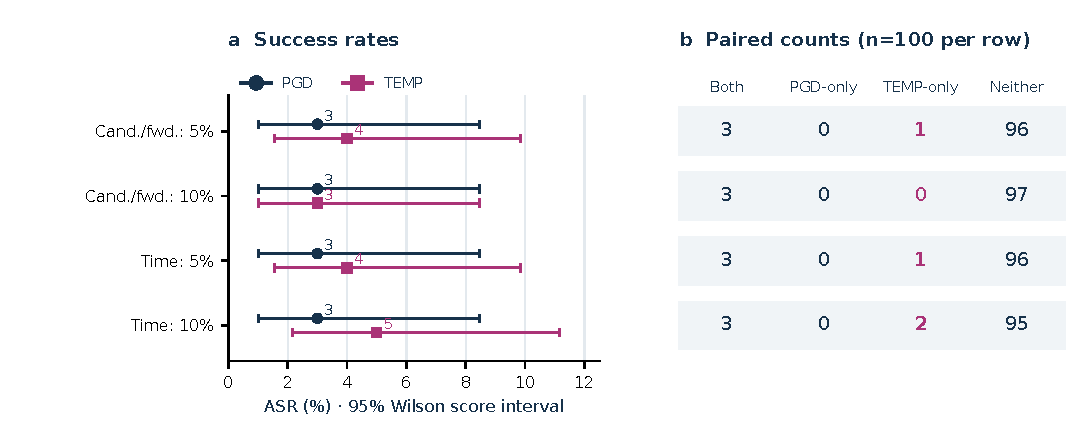
\includegraphics[width=\textwidth]{figures/fig02_matched_evaluation.pdf}
\caption{QSNN validation and paired timestamp attacks. (a) Five training seeds yield 97.272\% $\pm$ 0.212 percentage points (mean $\pm$ sample SD) on 5,000 validation examples. All runs share a split and pretrained frontend. (b--d) PGD/TEMP successes on the same 100 jointly clean-correct validation examples (seed 42); counts equal ASR percentages. Conditions match candidates, attack forwards, or calibrated elapsed time. Time matching uses TEMP Q=4,000 (QSNN) and 1,600 (SNN), with median TEMP/PGD timing ratios 0.978 and 1.083. All exact paired McNemar comparisons are nonsignificant; the largest discordance is b=0, c=2 (p=0.5). Backward costs are not equated by access matching. Sources: [R1, R3].}\label{fig:matched}
\end{figure*}

\subsection{Controlled packet-grid comparison}
The four-model grid study is separate from the timestamp experiment. It uses ten equal-event-count bins and amplitude-preserving packet retiming, with the same local training recipe, split, seed 42 and validation-selected checkpoint rule across architectures. Clean accuracy uses all 10,000 official-test examples. Each representation has its own frozen manifest of the first 1,000 examples correctly classified by all four models, selected from joint-correct pools of 9,522 binary and 9,495 integer examples. These common manifests are reused within representation for the two completed budgets, $B_\infty$ = 1 bin and B0 = 200 retimed packets.

On binary grids the custom SNN has 100.0\% and 99.5\% ASR under $B_\infty$ and B0, respectively. ConvNet has 1.9\% and 1.2\%, spiking ResNet18 has 0.1\% and 0.0\%, and VGGSNN has 0.0\% in both cells. Their full-test clean accuracies are 97.99\%, 96.90\%, 98.61\% and 99.21\%. On integer grids the corresponding ASR pairs are 99.9\%/98.0\%, 0.6\%/1.1\%, 0.2\%/0.1\% and 0.0\%/0.0\%, with clean accuracies of 98.14\%, 96.58\%, 98.12\% and 99.30\%. Each 0.1 ASR point represents one success among 1,000 attacked examples; the table gives all sixteen completed cells.

The largest reference-model ASR is descriptively 98.1 and 98.3 percentage points below the custom SNN for the binary budgets, and 99.3 and 96.9 points below it for the integer budgets. The integer-grid comparison supplies a particularly clear diagnostic: the custom SNN and spiking ResNet18 differ by only $0.02$ percentage points in clean test accuracy, but by $99.7$ and $97.9$ points in ASR under the two completed budgets. Similar clean accuracy therefore does not summarize the failure profile under this attack recipe. The source of the contrast remains unresolved, because a common recipe does not guarantee comparable optimization strength across architectures. In particular, zero observed successes should be read as failure of the evaluated attack on the selected examples, rather than as a robustness certificate \cite{athalye2018obfuscated,croce2020reliable}.

The source report states that every attack cell passed independent raw-data reconstruction and prediction audit. Common inputs and settings support a local architecture comparison without identifying the cause of the ASR gap. The campaign has one seed and two budgets; an unresolved B0 penalty discrepancy (5 attributed to the implementation by the report versus 10 in the reference paper) also limits replication claims. These local measurements must remain separate from published-reference tables, historical custom-SNN campaigns and the native-timestamp results.

Figure~\ref{fig:grid} shows the full 0--100\% outcome range and explicitly labeled control expansions. Table~\ref{tab:grid} gives every completed attack cell.

\begin{table*}[t]
\centering
\caption{Controlled four-model packet-grid results. Clean accuracy and ASR use different stated populations.}\label{tab:grid}
\small
\setlength{\tabcolsep}{4pt}
\renewcommand{\arraystretch}{1.16}
\begin{tabularx}{\linewidth}{L L C C C}
\toprule
\textbf{Grid} & \textbf{Architecture} & \textbf{Clean test \%} & \textbf{ASR $B_\infty$ = 1 \%} & \textbf{ASR $B_0$ = 200 \%}\\
\midrule
Binary & Custom SNN & 97.99 & 100.0 & 99.5\\
Binary & ConvNet & 96.90 & 1.9 & 1.2\\
Binary & Spiking ResNet18 & 98.61 & 0.1 & 0.0\\
Binary & VGGSNN & 99.21 & 0.0 & 0.0\\
Integer & Custom SNN & 98.14 & 99.9 & 98.0\\
Integer & ConvNet & 96.58 & 0.6 & 1.1\\
Integer & Spiking ResNet18 & 98.12 & 0.2 & 0.1\\
Integer & VGGSNN & 99.30 & 0.0 & 0.0\\
\bottomrule
\end{tabularx}
\vspace{3pt}
\begin{minipage}{\linewidth}\footnotesize Clean accuracy uses the complete 10,000-example official test set. ASR uses a separate frozen 1,000-example joint-correct manifest per representation. These are local measurements, not values copied from \cite{yu2026}. Source: [R4].\end{minipage}
\end{table*}

\begin{figure*}[t]
\centering
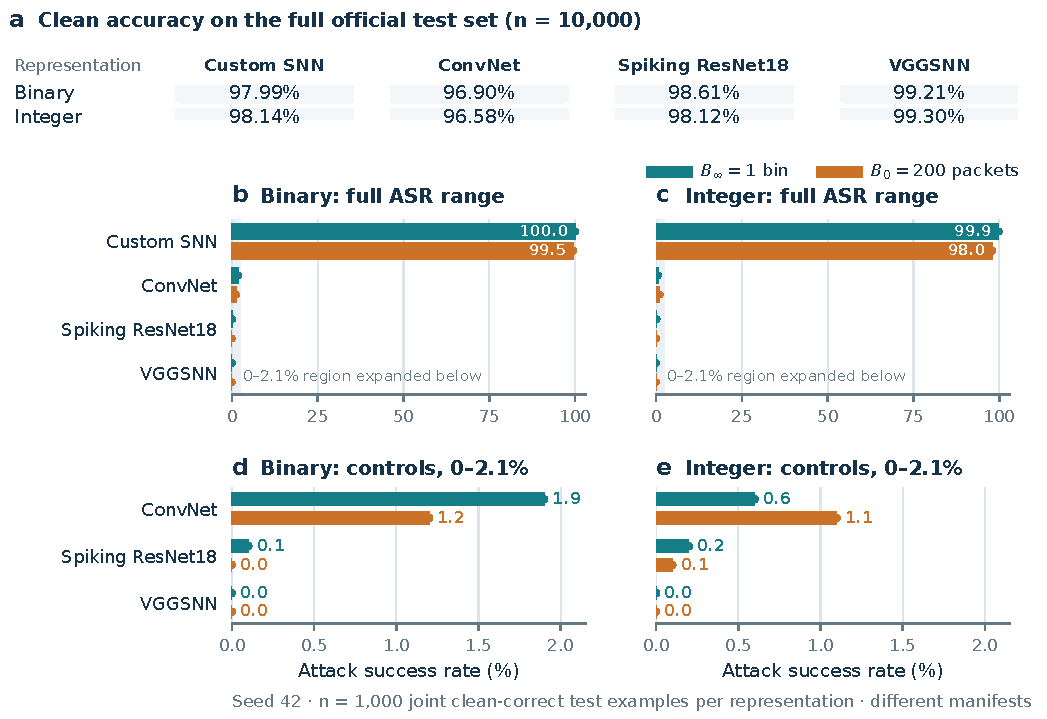
\includegraphics[width=\textwidth]{figures/fig03_grid_comparison.pdf}
\caption{Controlled local packet-retiming results (seed 42). (a) Clean accuracy uses all 10,000 official-test examples. (b,c) Full-range ASR under the two completed budgets; (d,e) declared expansions show the three controls at 0--2.1\%. Each attack cell uses 1,000 joint clean-correct test examples, so 0.1 percentage point is one success. Manifests are shared within each representation and differ between binary and integer. The local training and attack recipe is held constant across architectures. These single-seed, attack-specific results do not establish an architecture-independent ranking. The grid Custom SNN differs from the timestamp SNN. Source: controlled four-model report [R4].}\label{fig:grid}
\end{figure*}

\section{Discussion and limitations}\label{sec:discussion}
The experiments establish timing-only vulnerability in the implemented systems and show why the threat model and computational comparison are part of the result. The hybrid study identifies constrained retimings that change final predictions, while the classical grid study exhibits a large contrast under common local conditions. Their different samples, victims, representations and budget units prevent a single robustness ranking across the two studies.

The controlled architecture gap is the strongest observed contrast, but its mechanism remains unresolved. The integer custom SNN and spiking ResNet18 have nearly equal clean accuracy and radically different ASR, motivating direct investigation of temporal dynamics, decision geometry and architecture-dependent search difficulty. Shared nominal settings do not guarantee equally effective optimization. The low-ASR controls require stronger or adaptive attacks and independently trained seeds before a broader robustness conclusion is warranted.

The study does not isolate a quantum-specific failure mechanism. QSNN-v3 has a classical frontend and an analytically simulated circuit, and final TEMP-DRIFT-v2 optimizes class margin rather than quantum-state drift. Historical Iris diagnostics, retained in the supplement, show that greater mean state drift need not coincide with more classification failures. A mechanism study should relate final-model state distance to per-example outcomes while controlling clean margin and realized input distortion.

\paragraph{Encoding-aware interpretation.}
The quantum component is only one stage of the attacked composition. A feasible timestamp perturbation can change temporal aggregation, spiking summaries, encoded angles and the final probability vector. Without interventions that hold the frontend and training protocol fixed while replacing the readout, the observed failures cannot be attributed uniquely to quantum processing. This distinction complements comparisons of quantum and classical decision geometry \cite{wendlinger2024comparative} and avoids transferring guarantees between incompatible encoding or attacker-access settings \cite{gong2024randomized,dowling2026guarantees}.

\paragraph{Optimization diagnostics.}
The hard-forward, surrogate-backward timestamp pipeline makes attack diagnostics particularly relevant. Gradient checks, alternative surrogates, multiple initializations and gradient-free searches would help distinguish optimizer failure from difficult decision boundaries \cite{athalye2018obfuscated}. The principle of diverse attack evaluation \cite{croce2020reliable} is applicable, but an image-space ensemble cannot be imported unchanged: every candidate must obey the native event constraints or the packet-grid capacity rules. The present candidate and time controls are useful computational comparisons, not evidence that the search has exhausted either feasible set.

The remaining boundaries are concrete. Five hybrid seeds share one frontend and split; timestamp attacks reuse a selected validation population and one victim seed; grid attacks use deterministic joint-correct subsets. Official-test QSNN accuracy and robustness are absent. Tomography monitoring has no final N-MNIST detection or defense evaluation. This manuscript verifies report arithmetic rather than rerunning models or attacks, and original audit verdicts are attributed to the preserved reports because most underlying artifacts are missing.

\paragraph{Event preservation and stealth are distinct.}
An unchanged event count does not imply unchanged inter-spike intervals, frame histograms or detector behavior. The final-model experiments contain no statistical-indistinguishability test or adaptive attack against a deployed monitor. They are test-time evasion experiments; they do not modify a training set.

\paragraph{Next empirical steps.}
Future evaluation should select the final model using validation, then measure QSNN clean accuracy and attacks on the official test partition with independently trained frontend and head seeds, sample identifiers and each model's clean errors. Attack diagnostics should sweep restarts, iteration counts and step sizes, cross-entropy and margin losses, alternative surrogates and derivative-free budget curves. The best valid success found up to each budget should be recorded and reconfirmed with the hard forward pass.

A future component ablation should hold the frontend, split and training budget fixed while comparing a capacity-matched classical head and variational heads with and without entangling gates, reporting parameter counts and training costs. This ablation has not been performed. A state/margin study should retain each example's final state, probability vector and clean and attacked margins, comparing failures and survivors while controlling realized timestamp distortion and clean margin. Aggregate mean fidelity alone would not establish a mechanism.

The historical corrected integer campaign reports only 8 of 33 conditions complete. A proposed tomography monitor must first specify eight-qubit observables, a shot budget, clean-only calibration and a rejection or recovery policy, then measure ROC/PR curves, false-positive rates and adaptive-attack outcomes. These final-model defense results are unavailable. Local single-qubit marginals do not determine the full joint state. The supplementary mathematical analysis and earlier Iris diagnostics inform that proposal without supplying a final-model defense result.

\paragraph{Evidence availability.}
The comparison report contains results although its accompanying README states that no experiment results are present. We use the populated report and disclose this inconsistency. Most original checkpoints, raw per-example arrays, attack manifests and logs are absent from the accessible snapshot. We therefore distinguish checked report arithmetic from independently reproduced model runs and attribute the historical audit verdicts to their reports.

\section{Conclusion}\label{sec:conclusion}
QSNN-v3 provides an implemented eight-qubit hybrid victim with 97.272\% $\pm$ 0.212\% validation accuracy, and constrained timestamp retiming changes its decisions on 3--5 of the 100 examined joint-correct validation examples. Paired comparisons establish no significant advantage of TEMP-DRIFT-v2 over timestamp PGD; its largest numerical gain occurs under elapsed-time matching. In the separate common-recipe packet-grid study, the custom SNN exhibits 98.0--100\% ASR while three classical reference architectures exhibit 0--1.9\% under the two completed budgets. The resulting contribution is an explicit account of measurable retiming vulnerability within specified computational and representational settings. Official-test QSNN robustness, a quantum-specific failure mechanism and an effective final monitoring defense remain open empirical questions. The resulting evidence supports a protocol-specific account of end-to-end temporal vulnerability. It also identifies what stronger mechanistic claims would require: independent test evaluation, architecture-aware attack diagnostics, and per-example links between input distortion, quantum-state displacement and classification margin.

\section*{Data and code availability}
Implementation and preserved reports are available in the \texttt{ABC\_def1} repository \cite{repository}. The supplied supplement and data tables identify original report paths and the pinned snapshot. Tables transcribe available reports; they are not newly generated model outputs. Full experimental reproduction requires the omitted artifacts and original datasets. Author details are withheld for review, consistent with the supplied manuscript.

\bibliographystyle{unsrt}
\bibliography{references}
\end{document}
